\chapter{数学对象}
\label{chap:sets-functions-and-proofs}

设想我们记录了三次观测：输入分别为$1,2,3$，输出分别为$0,4,6$，
并希望用某条规则由输入预测输出。要把这件事写成可以计算和推理的形式，
至少要回答四个问题：允许哪些输入和输出；一条规则怎样把输入对应到输出；
候选规则有很多时怎样给它们编号、比较优劣；多次观测的数值怎样编号和汇总。

本章依次建立回答这些问题的对象。集合规定讨论范围，关系用有序对记录两个对象之间的联系；
索引族保留每次观测的编号，有限和、有限积与递推描述怎样汇总或逐项生成这些数值。
函数是一种特殊的关系，它为每个输入指定唯一输出；函数族与参数化则把许多候选规则组织起来。
比较候选规则时，常要问某个实数指标还能不能更小，这引出实数集合的界、确界与最值。
后续各章的计数、极限、微分、积分与优化都以这些对象和记号为起点。

\section{集合}
\label{sec:prelim-sets-relations-functions}

集合用来规定讨论对象的范围。例如，所有整数构成整数集合，某些满足条件的整数又可以组成其中的子集。

\subsection{集合的定义}
\label{sec:prelim-set-definition}

\paragraph{集合}
由一些确定的对象组成的整体称为\term{集合}（set），其中的对象称为元素。
若$x$是集合$X$的元素，记作$x\in X$；若不是，记作$x\notin X$。
例如$X=\{1,2,3\}$包含三个元素，有$2\in X$和$4\notin X$。

集合只由它包含哪些元素决定，不记录元素的排列次序和重复次数，
所以$\{1,2,3\}$、$\{3,2,1\}$和$\{1,1,2,3\}$表示同一个集合。

不含任何元素的集合称为空集，记作$\varnothing$。

\paragraph{集合的描述}
集合可以用列举法直接写出元素，如$A=\{1,2,3\}$。

条件法则给出集合中元素应满足的条件，如
\[
 A=\{i\in\mathbb Z:1\leq i\leq3\}.
\]
冒号读作“使得”，$\mathbb Z$表示整数集合。本书还用$\mathbb N$表示自然数集合
$\{0,1,2,\ldots\}$，用$\mathbb Q$和$\mathbb R$分别表示有理数集合与实数集合。

后面的区间记号约定：$[a,b]$包含两个端点，$(a,b)$不包含端点，
$[a,b)$与$(a,b]$各只包含一个端点。

\paragraph{子集}
若$A$的每个元素都属于$B$，就称$A$是$B$的子集（subset），记作$A\subseteq B$。
例如$\{1,2\}\subseteq\{1,2,3\}$。

每个集合都是自身的子集；空集没有元素，自然满足“每个元素都属于$B$”，所以是任何集合的子集。
若$A\subseteq B$且$A\neq B$，则称$A$是$B$的真子集，记作$A\subsetneq B$。

由于集合只由元素决定，$A=B$当且仅当$A\subseteq B$且$B\subseteq A$。
证明两个集合相等时，常把等式拆成这两个包含分别验证，称为双向包含。

成员关系与包含关系比较的对象不同：$1\in X$说明一个数属于$X$，
$\{1\}\subseteq X$说明一个集合的全部元素都在$X$中。

\paragraph{幂集}
集合$X$的全部子集组成的集合称为\term{幂集}（power set），记作
\[
 \mathcal P(X)=\{A:A\subseteq X\}.
\]
若$X=\{1,2\}$，则
$\mathcal P(X)=\{\varnothing,\{1\},\{2\},\{1,2\}\}$。
这里幂集的元素是集合；$\{1\}$是$\mathcal P(X)$的元素，$1$是$X$的元素。

\paragraph{集合族}
以集合为元素的集合称为集合族（family of sets）。
例如$\mathcal A=\{\{1\},\{2\}\}$是$X$的一个子集族，满足
$\mathcal A\subseteq\mathcal P(X)$，但它不等于整个幂集。
幂集收集全部子集，集合族则可以只收集所需的部分子集。

\subsection{集合的运算}
\label{sec:prelim-set-operations}

先固定本次讨论的全部对象，称为全集（universal set），取$U=\{1,2,3,4\}$。
再取其中两个集合$C=\{1,2,3\}$、$D=\{2,3,4\}$，下面几种运算都用它们作例子。

\paragraph{交集}
若要求一个对象同时满足两项成员条件，就取两个集合的交集：
\[
  X\cap Y=\{x:x\in X\text{ 且 }x\in Y\}.
\]
因此$C\cap D=\{2,3\}$，只保留同时属于$C$和$D$的元素。

\paragraph{并集}
若至少满足两项成员条件中的一项就允许保留，则取并集：
\[
  X\cup Y=\{x:x\in X\text{ 或 }x\in Y\}.
\]
这里的“或”包含两个条件同时成立的情形。
用上面的例子，$C\cup D=\{1,2,3,4\}=U$，因为全集中的每个元素至少属于
$C,D$中的一个；同时属于两者的$2,3$在并集中仍只出现一次。

\paragraph{差集}
若要求对象满足第一项成员条件，并排除满足第二项条件的对象，则取差集：
\[
  X\setminus Y=\{x:x\in X\text{ 且 }x\notin Y\}.
\]
因此$C\setminus D=\{1\}$，而$D\setminus C=\{4\}$，差集一般不能交换次序。

\paragraph{补集}
补集保留固定全集中不属于指定集合的对象。对$X\subseteq U$，定义
\[
  X^{\mathrm c}=U\setminus X.
\]
用上面的例子，$C^{\mathrm c}=\{4\}$。这个结果依赖事先固定的全集$U$：
若改以$\{1,2,3,4,5\}$为全集，同一个集合$C$的补集就变成$\{4,5\}$。
因此写补集时必须明确全集。

\subsection{集合运算的基本规律}
几种运算组合在一起时，需要知道哪些改写不改变结果。
交与并都可以交换次序、改变括号位置：
\[
 \begin{aligned}
  X\cap Y&=Y\cap X,&
  X\cup Y&=Y\cup X,\\
  (X\cap Y)\cap Z&=X\cap(Y\cap Z),&
  (X\cup Y)\cup Z&=X\cup(Y\cup Z).
 \end{aligned}
\]
它们来自“且”“或”两个连接词本身的交换与结合规律。

交与并之间还互相分配：
\[
 X\cap(Y\cup Z)=(X\cap Y)\cup(X\cap Z),\qquad
 X\cup(Y\cap Z)=(X\cup Y)\cap(X\cup Z).
\]
以第一式为例，左边要求$x\in X$，并且$x$属于$Y$或$Z$；这恰好是说$x$同时属于$X$与$Y$，
或者同时属于$X$与$Z$。第二式可以同样逐字改写。

补集与交、并的关系称为De Morgan律：对全集$U$中的子集$X,Y$，
\begin{equation}
 (X\cup Y)^{\mathrm c}=X^{\mathrm c}\cap Y^{\mathrm c},\qquad
 (X\cap Y)^{\mathrm c}=X^{\mathrm c}\cup Y^{\mathrm c}.
 \label{eq:prelim-de-morgan-two-sets}
\end{equation}

下面用双向包含验证第一式。若$u\in(X\cup Y)^{\mathrm c}$，则$u$既不属于$X$也不属于$Y$，
否则它会落在并集中；因此$u\in X^{\mathrm c}\cap Y^{\mathrm c}$。反过来，若$u$同时属于两个补集，
它就不属于$X$、也不属于$Y$，从而不属于$X\cup Y$。两个方向合起来便是等式。
第二式的论证相同：不属于$X\cap Y$，就是至少不属于$X,Y$中的一个。

用前面的例子核对：$C\cup D=U$，故左边为空集；右边$C^{\mathrm c}\cap D^{\mathrm c}=\{4\}\cap\{1\}$也是空集。
De Morgan律说明，“不满足任一条件”与“每个条件都不满足”是同一件事；
后面计数不满足限制的对象、构造可测集合时都会用到它。

\section{关系}
\label{sec:prelim-binary-relations}

集合规定了对象的范围，接下来要记录两个对象之间的联系。
例如“输入$2$对应观测输出$4$”“$1$不大于$2$”“两个整数除以$2$的余数相同”，
都可以表示为一对对象是否满足某个条件。本节先定义二元关系及其性质，
再讨论怎样补全这些性质，以及怎样用等价关系分组、用偏序关系比较对象。

\subsection{二元关系}
\label{sec:prelim-binary-relation-definition}

\paragraph{有序对}
记录两个对象时，常常需要区分谁在前、谁在后。
有序对$(x,y)$保留两个位置：第一个位置放$x$，第二个位置放$y$；
两个有序对相等，即$(x,y)=(x',y')$，要求$x=x'$且$y=y'$。
所以$(1,2)\neq(2,1)$，而作为集合的$\{1,2\}$与$\{2,1\}$相等。

本章开头的一次观测可以写成$(x,y)$，第一个位置记录输入，第二个位置记录观测输出；
三次观测就是$(1,0)$、$(2,4)$、$(3,6)$三个有序对。

\paragraph{笛卡尔积}
若第一个位置的对象取自集合$X$，第二个位置的对象取自集合$Y$，
全部可能的有序对组成两个集合的\term{笛卡尔积}（Cartesian product）：
\[
 X\times Y=\{(x,y):x\in X,\ y\in Y\}.
\]
例如$\{1,2\}\times\{a,b\}=\{(1,a),(1,b),(2,a),(2,b)\}$。
当$X,Y$都非空且$X\neq Y$时，$X\times Y\neq Y\times X$：两个位置的取值范围交换了，
例如$(1,a)$属于上面的积，却不属于$\{a,b\}\times\{1,2\}$。

同样可以定义由$d$个位置组成的笛卡尔积，其元素是有序的$d$元组。
特别地，记$\mathbb R^d=\mathbb R\times\cdots\times\mathbb R$（共$d$个因子），
其中每个元素是一个有序的$d$元实数组$(x_1,\ldots,x_d)$；$\mathbb R^2$就是平面上全部点的坐标。

\paragraph{二元关系}
笛卡尔积列出了全部可能的对，但一个具体条件通常只被其中一部分对满足。
把满足条件的对收集起来，这个子集就完整记录了该条件。

设$X,Y$是两个集合。笛卡尔积的任一子集$R\subseteq X\times Y$
称为$X$到$Y$的\term{二元关系}（binary relation）；写$xRy$表示$(x,y)\in R$，读作“$x$与$y$有关系$R$”。
$X=Y$时，称$R$为$X$上的关系。

例如实数上的“不大于”关系是$R=\{(x,y)\in\mathbb R^2:x\leq y\}$；
$(1,2)$属于$R$，$(2,1)$却不属于，所以$1R2$不意味着$2R1$。
有序对规定了方向，但这不排除某些关系本身对两个方向一视同仁，例如“相等”关系。

二元关系也不要求每个$x$恰好关联一个$y$：同一个$x$可以关联多个$y$，也可以不关联任何$y$。

由于每个关系都是$X\times Y$的子集，$X$到$Y$的全部关系组成的集合恰是幂集$\mathcal P(X\times Y)$；
空集与整个笛卡尔积也都是关系，分别表示“没有任何一对满足条件”与“每一对都满足条件”。

\subsection{关系的性质}
\label{sec:prelim-relation-properties}

同样是集合上的关系，“相等”“严格小于”和“不大于”遵守的规则并不相同。
下面固定集合$X$上的关系$R\subseteq X\times X$，依次考察三种情形：对象与自身是否有关系，
交换两个对象的位置后关系是否保持，以及经过中间对象的关系能否直接得到。

\paragraph{自反性与反自反性}
若每个$x\in X$都有$xRx$，称$R$具有\term{自反性}（reflexivity），也称反身性。
若每个$x\in X$都不满足$xRx$，称$R$具有\term{反自反性}（irreflexivity）。
实数上的$\leq$是自反的，$<$是反自反的。
不具有自反性只表示至少有一个对象不与自身关联，并不意味着所有对象都不与自身关联。
例如在$X=\{1,2\}$上，$R=\{(1,1)\}$既不自反，也不反自反。

\paragraph{对称性与反对称性}
若对任意$x,y\in X$，$xRy$都蕴含$yRx$，称$R$具有\term{对称性}（symmetry）。
若$xRy$且$yRx$只能在$x=y$时同时成立，称$R$具有\term{反对称性}（antisymmetry）。
“余数相同”是对称的，“不大于”是反对称的。
反对称性并非对称性的否定：对称性允许两个不同对象互相关联，反对称性则要求双向关联只出现在同一个对象上。
相等关系同时具有两种性质，因为它只关联同一个对象。

\paragraph{传递性}
若对任意$x,y,z\in X$，由$xRy$且$yRz$总能推出$xRz$，
称$R$具有\term{传递性}（transitivity）。例如$x\leq y$且$y\leq z$蕴含$x\leq z$。
传递性要求经过中间对象得到的联系也直接属于关系；它与交换两个对象的位置无关。

\paragraph{关系的闭包}
一个关系可能尚未满足所需性质。若只允许加入有序对，就可以寻找包含原关系、
具有指定性质且在包含意义下最小的关系，称为相应的\term{关系闭包}（closure of a relation）。
这里的“最小”是说：任何包含原关系并具有该性质的关系都包含它。
下面对自反、对称和传递三种性质分别构造闭包。

令$\Delta_X=\{(x,x):x\in X\}$，则自反闭包为$R\cup\Delta_X$：补上所有缺少的自身关联即可。
令$R^{-1}=\{(y,x):(x,y)\in R\}$，则对称闭包为$R\cup R^{-1}$：为每一对补上反向的对。
两种构造都满足对应性质，而且任何包含$R$并具有该性质的关系都必须包含补入的对。

传递闭包记作$R^+$。规定$xR^+y$当且仅当存在正整数$n$及对象
$x=x_0,x_1,\ldots,x_n=y$，使每个$k=1,\ldots,n$都有$x_{k-1}Rx_k$。
也就是说，沿原关系连续走有限步能够到达的两个对象，在$R^+$中直接关联。
把两条这样的有限链首尾相接，仍得到有限链，因此$R^+$具有传递性；
另一方面，任何包含$R$的传递关系沿链逐步应用传递性，都必须包含每条有限链的首尾对。
所以$R^+$确实是包含$R$的最小传递关系。

例如在$X=\{1,2,3\}$上取$R=\{(1,2),(2,3)\}$，自反闭包补入三个$(i,i)$，
对称闭包补入$(2,1),(3,2)$，传递闭包只需补入$(1,3)$。
$R^+$不一定包含所有$(x,x)$；再并入$\Delta_X$才得到自反传递闭包$R^*$。

反对称性则不能总靠添加有序对获得：若原关系已含两个不同对象之间的双向关联，
任何扩充都仍保留这对违反条件的有序对。

\subsection{等价关系}
\label{sec:prelim-equivalence-relations}

\paragraph{等价关系}
要按某个标准把对象分组，例如按除以$2$的余数把整数分成偶数和奇数，
可以先写出“两个对象属于同一组”这一关系，再问它需要满足什么条件。
首先，每个对象都应与自己同组；其次，若$x$与$y$同组，则$y$与$x$也同组；
最后，若$x$与$y$同组、$y$与$z$同组，则$x$与$z$也应同组，否则是否“同组”会随所经过的中间对象而改变。
下面把这三条要求写成定义。

\begin{definition}[等价关系]
\label{def:prelim-equivalence-relation}
设$R$是集合$X$上的关系。若对任意$x,y,z\in X$都有
\begin{itemize}
  \item $xRx$；
  \item $xRy$蕴含$yRx$；
  \item $xRy$且$yRz$蕴含$xRz$，
\end{itemize}
就称$R$为\term{等价关系}（equivalence relation），即能够把对象按同一标准分组的关系。
三条性质依次是前面定义的反身性（自反性）、对称性与传递性。
\end{definition}
按余数分组时，整数上的关系“$x-y$能被$2$整除”满足三条性质：$x-x=0$能被$2$整除；
$x-y$能被$2$整除时$y-x$也能；$x-y$与$y-z$都能被$2$整除时，它们的和$x-z$也能。

\paragraph{等价类}
有了等价关系，就能把与某个对象等价的全部对象收集为一组。
给定$x\in X$，与$x$等价的对象组成它的\term{等价类}（equivalence class）
\[
 [x]_R=\{y\in X:yRx\}.
\]
在余数的例子中，$[0]_R$是全部偶数，$[1]_R$是全部奇数，而$[2]_R=[0]_R$：
同一个等价类可以由不同的代表元写出。

我们还要确认，等价类确实把$X$分成了互不重叠、合起来又不遗漏的若干组。
把这一要求写清楚：若$X$的一族非空子集两两不交，并且它们的并等于$X$，就称这族子集为$X$的一个\term{划分}（partition）。
下面证明全部等价类组成$X$的一个划分。

其一，反身性给出$x\in[x]_R$，所以每个等价类非空，并且每个对象至少属于一个等价类，全部等价类的并就是$X$。
其二，两个等价类要么相等，要么不交。设$z$同属$[x]_R$与$[y]_R$，则$zRx$与$zRy$成立；
由对称性把$zRx$翻成$xRz$，再与$zRy$用传递性得到$xRy$。
有了$xRy$，任取$u\in[x]_R$就有$uRx$，再由传递性得$uRy$，即$u\in[y]_R$，于是$[x]_R\subseteq[y]_R$；
交换$x$与$y$的位置又得到$[y]_R\subseteq[x]_R$。所以$[x]_R=[y]_R$。
这说明只要两个等价类有一个公共元素，它们就完全相同，因而不可能只重叠一部分。

反过来，任给$X$的一个划分，规定“$x$与$y$属于划分中的同一块”，就得到一个等价关系，
它的等价类正是划分中的各块。因此在同一个集合上，“给出等价关系”与“给出划分”是同一件事的两种写法。

\paragraph{商集}
分组以后，我们常把每一组当作一个新的对象来讨论。
全部等价类组成的集合记为$X/R$，称为商集（quotient set）。
例如按除以$2$的余数对整数分类，商集中只有偶数类和奇数类两个元素；
商集的元素是等价类，即原集合的子集，而不是原来的整数。

再看平面中除原点以外的点。规定两个点等价，当且仅当它们位于同一条过原点的直线上。
用坐标表示，$P=(p_1,p_2)$与$Q=(q_1,q_2)$等价，
就是存在非零实数$c$使$p_1=cq_1$、$p_2=cq_2$，下面简记为$P=cQ$。
三条性质可以逐一验证：取$c=1$得到反身性；若$P=cQ$，则$Q=(1/c)P$，得到对称性；
若$P=cQ$且$Q=c'S$，则$P=(cc')S$且$cc'\neq0$，得到传递性。
每个等价类是一条过原点的直线去掉原点，商集的元素就对应这些直线。

若只允许$c>0$，三条性质仍然成立（$1/c$与$cc'$仍为正数），但同一直线在原点两侧的部分分属不同的类，
每个类是一条从原点出发、不含原点的射线。
图~\ref{fig:vol1-add-equivalence-directions}用从原点出发的箭头标记这些点，
比较是否区分朝向时的两种分类。
\begin{figure}[!htb]
  \centering
  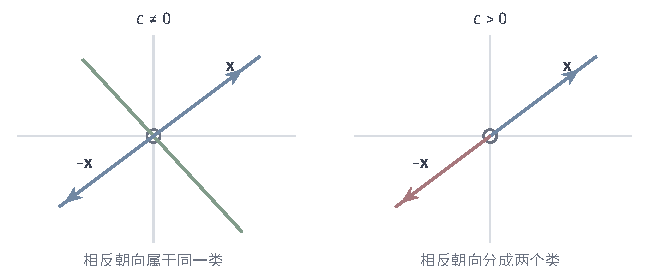
\includegraphics[width=112mm]{figures/01-mathematical-preliminaries-upper/00-shared/tikz/mathematical-language-combinatorics-analysis-optimization-comprehension-additions/equivalence-directions.pdf}
  \caption{平面中非原点的等价分类。每支箭头从原点指向一个点。左侧允许非零实比例，同一直线上的点属于同一类；右侧只允许正比例，同一直线的两侧分成蓝、红两类。绿色表示另一条直线上的类；空心原点不属于被分类的集合。}
  \label{fig:vol1-add-equivalence-directions}
\end{figure}

\subsection{偏序关系}
\label{sec:prelim-order-relations}

\paragraph{偏序与全序}
等价关系把对象分组，另一类常见的关系则用来比较先后或大小。
实数上的$\leq$可以比较任意两个数；集合之间的包含关系却不一定。
在$\mathcal P(\{1,2\})$中，$\varnothing\subseteq\{1\}\subseteq\{1,2\}$，
但$\{1\}$和$\{2\}$互不包含。包含关系可以比较其中一些对象，却不能比较任意两个对象。
下面的定义提炼出这类比较关系共同满足的条件。
\begin{definition}[偏序关系]
\label{def:prelim-partial-order}
集合$X$上的\term{偏序关系}（partial order）$R$是一种允许部分对象互不可比的比较关系：
它对任意$x,y,z\in X$满足反身性$xRx$、传递性（$xRy$且$yRz$蕴含$xRz$），
以及反对称性（$xRy$且$yRx$时必有$x=y$）。
若任意两个元素还至少满足$xRy$或$yRx$中的一个，则称$R$为全序（total order）。
\end{definition}
实数上的$\leq$是全序，因为任意两个实数都可比较。
幂集上的$\subseteq$是偏序：每个集合包含自身，包含关系可以传递，双向包含意味着集合相等；
但它不是全序，因为$\{1\}$与$\{2\}$互不包含。

\paragraph{最小元与最大元}
配备了偏序关系的集合称为偏序集合，记作$(X,\preceq)$，其中$\preceq$表示所选的偏序关系；
实数大小、集合包含等都可作为它的具体解释。
对非空子集$A\subseteq X$，若$a_{\min}\in A$满足$a_{\min}\preceq a$对每个$a\in A$成立，
就称$a_{\min}$为$A$的\term{最小元}（least element）。
若$a_{\max}\in A$满足$a\preceq a_{\max}$对每个$a\in A$成立，
就称$a_{\max}$为$A$的\term{最大元}（greatest element）。
若最小元存在，它必唯一：两个最小元彼此都不大于对方，由反对称性只能相等；最大元同理。

例如在$(\mathcal P(\{1,2\}),\subseteq)$中，整个幂集的最小元是$\varnothing$，最大元是$\{1,2\}$。
但子集族$\{\{1\},\{2\}\}$没有最小元，也没有最大元，因为两者互不可比。

\paragraph{极小元与极大元}
最小元要能与集合中的所有元素比较。若只要求$A$中没有比$a\in A$严格更小的元素，
即$b\in A$且$b\preceq a$必有$b=a$，就称$a$为\term{极小元}（minimal element）。
类似地，若$b\in A$且$a\preceq b$必有$b=a$，就称$a$为\term{极大元}（maximal element）。
最小元一定是极小元，反过来未必成立；最大元与极大元也有相同区别。
在刚才的子集族$\{\{1\},\{2\}\}$中，两个元素都是极小元，也都是极大元，
却都不是最小元或最大元。在全序中任意两元素可比，所以极小元必为最小元，极大元必为最大元。

\paragraph{上界与下界}
最小元和最大元必须属于$A$。若放宽这一要求，允许比较的基准取在$A$以外，就得到界；
不过界仍须属于事先选定的偏序集合$X$。
若$u\in X$满足$a\preceq u$对每个$a\in A$成立，称$u$为$A$的\term{上界}（upper bound）；
若$l\in X$满足$l\preceq a$对每个$a\in A$成立，称$l$为$A$的\term{下界}（lower bound）。
例如对$A=\{\{1\},\{2\}\}\subseteq\mathcal P(\{1,2\})$，
$\varnothing$是下界，$\{1,2\}$是上界，它们都不属于$A$。
因此存在上下界不意味着存在最小元和最大元；反过来，属于$A$的下界就是最小元，属于$A$的上界就是最大元。

\paragraph{上确界与下确界}
若$A$的全部上界组成的集合有最小元，就称它为$A$的上确界，记为$\sup A$；
若全部下界组成的集合有最大元，就称它为$A$的下确界，记为$\inf A$。
在幂集的包含偏序下，子集族的并是上确界，交是下确界：并包含每个成员，因而是上界，
又包含于任何一个共同上界，因而是最小的上界；交的论证方向相反。
于是前例中$\sup A=\{1,2\}$、$\inf A=\varnothing$，但$A$仍无最大元和最小元。
一般偏序集合不保证这些确界存在；第~\ref{sec:prelim-optimal-values-errors}节将在实数中用完备性保证非空有界集合的确界存在。

\section{索引族}
\label{sec:prelim-indices-sums-recurrences}

同一个数可以在一组记录中出现多次。例如记录$(1,1,4)$有三项，取值集合却只有$\{1,4\}$。
本节先用编号保留每次出现，再讨论怎样对这些带编号的对象求和、求积或逐项生成。

\subsection{索引族与序列}
\label{sec:prelim-indexed-sequences}

\paragraph{索引族}
直接把记录组成集合，会丢掉重复值所在的位置。为此给每项记录一个编号，并为每个编号指定唯一的对象。

\begin{definition}[索引族]
\label{def:prelim-indexed-family}
给定索引集合$I$和对象集合$X$，若为每个$i\in I$指定唯一的对象$a_i\in X$，就得到索引族（indexed family）。
整个族写作$(a_i)_{i\in I}$；也可把第$i$项记作$a(i)$。
\end{definition}
开头的记录写成索引族就是$a_1=1,a_2=1,a_3=4$，共有三个编号；
虽然前两个编号对应相同的数，求和时仍应分别计入。
索引集合未必有顺序，例如用城市名索引一组气温时，城市名本身没有规定先后。

\paragraph{序列}
按正整数顺序索引的对象族称为序列（sequence）。
若只取$1,\ldots,n$，就得到有限序列；若取全部正整数，就得到无限序列。
取值为实数的序列称为数列，例如$(1/n)_{n\geq1}$。
序列还可以从$0$开始，此时明写$(a_n)_{n\geq0}$。
带下标的对象族不一定是序列；序列的先后顺序来自整数索引本身的大小顺序。

序列也可以记录逐步更新的结果。若第$t$步的结果还包含多个坐标，就把第$j$个坐标记作$a_j^{(t)}$，其中带括号的上标$t$表示迭代步。
普通上标仍表示幂，所以$a_j^2$与$a_j^{(2)}$不同。

\paragraph{二维索引族}
一项观测含有多个坐标时，需要同时保留观测编号与坐标编号，可以用两个索引共同指定一个对象。
给定索引集合$I,J$及对象集合$X$，为每个$(i,j)\in I\times J$指定唯一对象$a_{i,j}\in X$，就得到二维索引族，
整个族写作$(a_{i,j})_{(i,j)\in I\times J}$。
只有两个索引都确定以后，才指定出一个对象；固定其中一个索引，就得到由另一个索引编号的一族对象。
例如$I=\{1,2\}$、$J=\{1,2,3\}$，令$a_{i,j}=3(i-1)+j$，可排成
\[
 \begin{array}{c@{\quad}ccc}
  &j=1&j=2&j=3\\\hline
 i=1&1&2&3\\
 i=2&4&5&6
 \end{array}.
\]
此时$a_{2,3}=6$；固定$i=2$得到第二行的三项，固定$j=2$得到第二列的两项。
本书在多维索引间写逗号，并在每次使用时说明各索引的范围。

\subsection{集合族的并与交}
\label{sec:prelim-indexed-set-operations}
索引族中的对象也可以是集合。给定索引族$(A_i)_{i\in I}$，其中每个$A_i$都是全集$U$的子集，
两个集合的并与交可以推广到任意多个集合：
\[
 \begin{aligned}
  \bigcup_{i\in I}A_i
  &=\{u\in U:\text{存在 }i\in I\text{ 使 }u\in A_i\},\\
  \bigcap_{i\in I}A_i
  &=\{u\in U:\text{对每个 }i\in I\text{ 都有 }u\in A_i\}.
 \end{aligned}
\]
$I=\{1,2\}$时回到前面的$A_1\cup A_2$与$A_1\cap A_2$；
$I=\{1,2,\ldots\}$时也写成$\bigcup_{n=1}^\infty A_n$。
例如在全集$U=[0,1]$中取$A_n=[1/n,1]$，则$\bigcup_{n\geq1}A_n=(0,1]$：
每个$x\in(0,1]$在$n\geq1/x$时属于$A_n$，而$0$不属于任何$A_n$。

De Morgan律对任意索引族同样成立：
\begin{equation}
 \begin{aligned}
  \left(\bigcup_{i\in I}A_i\right)^{\mathrm c}
  &=\bigcap_{i\in I}A_i^{\mathrm c},\\
  \left(\bigcap_{i\in I}A_i\right)^{\mathrm c}
  &=\bigcup_{i\in I}A_i^{\mathrm c}.
 \end{aligned}
 \label{eq:prelim-de-morgan-families}
\end{equation}
证明与两个集合时相同：$u$不属于并集，等价于对每个$i$都不属于$A_i$；
$u$不属于交集，等价于至少有一个$i$使$u\notin A_i$。
后面测量集合时要对一列无穷多个集合取并与交，用的就是这里的记号和规律。

\subsection{有限和与有限积}
\label{sec:prelim-finite-sums-products}

\paragraph{有限和与有限积}
对$n\geq1$个实数$a_1,\ldots,a_n$，依次相加与相乘分别记为
\[
  \sum_{i=1}^{n}a_i=a_1+\cdots+a_n,\qquad
  \prod_{i=1}^{n}a_i=a_1\cdots a_n.
\]
例如$a_1=1,a_2=4,a_3=9$时，有限和为$14$，有限积为$36$。
若没有任何项，约定
\[
  \sum_{i\in\varnothing}a_i=0,\qquad
  \prod_{i\in\varnothing}a_i=1.
\]
理由是把一组项拆成两部分分别汇总时，若其中一部分为空，结果不应改变：加法需要$0$，乘法需要$1$。
例如从累计值$0$开始逐项相加，尚未加入任何一项时的累计值正好是空和。

\paragraph{哑索引与自由索引}
范围确定后，求和变量的名称不影响结果：
\[
  \sum_{i=1}^{n}a_i=\sum_{k=1}^{n}a_k.
\]
这里$i$是\term{哑索引}（dummy index），它只是“当前加到第几项”的占位记号，
求和完成后不再出现，所以换成任何没在别处用过的字母，结果都不变。

自由索引则不同。设$x_{i,j}$表示第$i$个样本的第$j$个坐标，把$n$个样本的同一坐标加起来，得到
\[
  b_j=\sum_{i=1}^{n}x_{i,j},\qquad j=1,\ldots,d.
\]
其中$j$是自由索引（free index）：固定$j$才能知道在汇总哪个坐标，它也出现在结果$b_j$中。
可以把求和的$i$统一改为$k$，却不能只把右侧的$j$改成$k$而保留左侧的$b_j$。
给哑索引换名时，也不能占用式中已有的自由索引；把本式的$i$改成$j$会破坏原来的含义。

\paragraph{有限和的运算法则}
有限和中的各项可以先乘系数再相加，也可以先分别求和再乘系数。这一规则称为求和的线性关系，
它来自实数加法的交换律、结合律以及乘法对加法的分配律。对实数$a,b$与实数$u_1,\ldots,u_n$、$v_1,\ldots,v_n$，
\[
  \sum_{i=1}^{n}(au_i+bv_i)
  =
  a\sum_{i=1}^{n}u_i+b\sum_{i=1}^{n}v_i.
\]

\paragraph{有限积的运算法则}
有限积可以按对应项相乘后合并，也可以把同一个常数从每一项中提出。对$n\geq1$个实数
$a_i,b_i$和实常数$c$，有
\[
 \prod_{i=1}^n(a_i b_i)
 =\left(\prod_{i=1}^n a_i\right)\left(\prod_{i=1}^n b_i\right),\qquad
 \prod_{i=1}^n(ca_i)=c^n\prod_{i=1}^n a_i.
\]
这些等式来自实数乘法的交换律与结合律；第二式中$c$共出现$n$次。
若每个$b_i\neq0$，还可逐项相除：
\[
 \prod_{i=1}^n\frac{a_i}{b_i}
 =\frac{\prod_{i=1}^n a_i}{\prod_{i=1}^n b_i}.
\]
例如$(2\cdot1)(2\cdot4)(2\cdot9)=2^3(1\cdot4\cdot9)=288$。

有限积没有类似求和的线性关系。取$a_1=1,b_1=2,a_2=3,b_2=4$，则
$\prod_{i=1}^2(a_i+b_i)=(1+2)(3+4)=21$，而$\prod_{i=1}^2a_i+\prod_{i=1}^2b_i=1\cdot3+2\cdot4=11$，
所以一般不能把和的连乘拆成两个连乘之和。

\paragraph{多重求和}
对有限实数数组$(a_{i,j})$，$i=1,\ldots,n$，$j=1,\ldots,d$，可以先按行求和，也可以先按列求和：
\[
  \sum_{i=1}^{n}\sum_{j=1}^{d}a_{i,j}
  =
  \sum_{j=1}^{d}\sum_{i=1}^{n}a_{i,j},
\]
因为两边都遍历$\{1,\ldots,n\}\times\{1,\ldots,d\}$，每个索引对恰好贡献一次；
有限实数加法的交换律和结合律允许改变遍历顺序。
例如数组两行为$(1,2,3)$和$(4,5,6)$，按行汇总得$6+15=21$，
按列汇总得$5+7+9=21$。

如果内层范围依赖外层索引，换序时范围也必须随之重写。例如
\begin{equation}
  \sum_{i=1}^{n}\sum_{j=1}^{i}a_{i,j}
  =
  \sum_{j=1}^{n}\sum_{i=j}^{n}a_{i,j}.
  \label{eq:prelim-triangular-sum}
\end{equation}
两边遍历的索引对都恰好是满足$1\leq j\leq i\leq n$的全部$(i,j)$。$n=3$时共有六项，
分别对应$(1,1)$、$(2,1)$、$(2,2)$、$(3,1)$、$(3,2)$和$(3,3)$。
若把右侧内层误写为$i=1,\ldots,n$，就会遍历全部九个索引对，多算$(1,2)$、$(1,3)$、$(2,3)$三项。
合法换序保留的是同一批项，不只是交换两个求和符号。
无限级数与积分的换序还需要额外条件，不能仅从有限情形类推。

\paragraph{多重求积}
对有限实数数组$(a_{i,j})$，把每个位置的数各乘一次，得到多重积。
由于乘法满足交换律与结合律，矩形索引范围内可以按行或按列求积：
\[
 \prod_{i=1}^n\prod_{j=1}^d a_{i,j}
 =\prod_{j=1}^d\prod_{i=1}^n a_{i,j}.
\]
例如两行为$(1,2,3)$和$(4,5,6)$时，两种次序分别给出
\[
 (1\cdot2\cdot3)(4\cdot5\cdot6)
 =(1\cdot4)(2\cdot5)(3\cdot6)=720.
\]
与多重求和一样，内层范围依赖外层索引时，换序必须保留同一批索引对。例如
\[
 \prod_{i=1}^n\prod_{j=1}^i a_{i,j}
 =\prod_{j=1}^n\prod_{i=j}^n a_{i,j}.
\]
两边都只取满足$1\leq j\leq i\leq n$的位置；这些有限积的换序不要求各项非零。

\subsection{递推关系}
\label{sec:prelim-recurrence-unrolling}

\paragraph{递推关系}
从初值出发、用已经得到的项确定下一项的关系称为\term{递推}（recurrence）。
例如对$a_1=1,a_2=4,a_3=9$，累计和可以写成
\[
 S^{(0)}=0,\qquad S^{(t+1)}=S^{(t)}+a_{t+1},\qquad t=0,1,2.
\]
依次得到$S^{(1)}=1$、$S^{(2)}=5$、$S^{(3)}=14$。
同一组数也可写为$S^{(t)}=\sum_{i=1}^t a_i$：求和式直接给出第$t$项，
递推式则说明如何从前一项得到后一项。初值与更新关系共同确定序列；只有更新关系通常不够。

\paragraph{数学归纳法}
由递推猜出通项公式以后，需要确认公式对\emph{每一个}$t$都成立，而不只对算过的前几项成立。
递推式本身提示了证明方法：若公式在初值处成立，并且“公式对第$t$项成立”总能推出“它对第$t+1$项成立”，
那么从初值出发逐步推进，任何给定的$t$都能在有限步内到达，公式便对全部$t$成立。

这种证明方法称为\term{数学归纳法}（mathematical induction）：要证明关于$t=0,1,2,\ldots$的命题$P(t)$全部成立，
只需证明$P(0)$成立（归纳基础），以及对每个$t\geq0$，由$P(t)$可推出$P(t+1)$（归纳步）。
归纳步中暂时假定的$P(t)$称为归纳假设。

以前面的累计和为例，命题$P(t)$为$S^{(t)}=\sum_{i=1}^ta_i$。
$P(0)$成立，因为$S^{(0)}=0$恰是空和。若$P(t)$成立，则
$S^{(t+1)}=S^{(t)}+a_{t+1}=\sum_{i=1}^ta_i+a_{t+1}=\sum_{i=1}^{t+1}a_i$，即$P(t+1)$成立。
所以递推式与求和式对每个$t$描述同一个序列。

\paragraph{等差递推}
若每一步都增加同一个实数$d$，就得到等差递推：
\[
 a^{(t+1)}=a^{(t)}+d,\qquad a^{(0)}=a_0,\qquad t=0,1,\ldots.
\]
从初值到第$t$步共加了$t$次$d$，因此
\[
 a^{(t)}=a_0+td.
\]
用归纳法写出来：$t=0$时右侧为$a_0$；若$a^{(t)}=a_0+td$，则$a^{(t+1)}=a_0+td+d=a_0+(t+1)d$。
例如从$2$开始，每步加$3$，依次得到$2,5,8,11,\ldots$，第$t$步为$2+3t$。
$d>0$时各项递增，$d<0$时各项递减，$d=0$时保持初值。

\paragraph{等比递推}
从$8$开始，每一步乘$1/2$，便依次得到$8,4,2,1,\ldots$。
用$e^{(t)}$表示第$t$项，把$1/2$推广为固定系数$\rho\in\mathbb{R}$，可写成
\begin{equation}
  e^{(t+1)}=\rho e^{(t)},\qquad e^{(0)}=e_0,\qquad t=0,1,\ldots,
  \label{eq:prelim-geometric-recurrence}
\end{equation}
逐步展开得到
\[
  e^{(t)}=\rho^t e_0,\qquad t=0,1,2,\ldots
\]
（约定$\rho^0=1$）。归纳步只需一行：若$e^{(t)}=\rho^te_0$，则$e^{(t+1)}=\rho\cdot\rho^te_0=\rho^{t+1}e_0$。
每步都有$|e^{(t+1)}|=|\rho|\,|e^{(t)}|$：当$|\rho|<1$时，非零项的绝对值在下一步缩小；
$\rho=-1$使大小不变而符号交替，$|\rho|>1$使非零项的绝对值放大。
若$e_0=0$，每一项都是零；若$\rho=0$，第一次更新后便一直为零。

\paragraph{有限几何和}
等比序列的各项相加，得到有限几何和$G_N=\sum_{n=0}^N\rho^n=1+\rho+\cdots+\rho^N$。
它可以用“错位相减”求出：把$G_N$乘以$\rho$，每一项都向后移一位，
\[
 \rho G_N=\rho+\rho^2+\cdots+\rho^{N+1}.
\]
两式相减时，中间各项成对抵消，只剩首项$1$与末项$\rho^{N+1}$：$(1-\rho)G_N=1-\rho^{N+1}$。因此
\begin{equation}
 \sum_{n=0}^N\rho^n=\frac{1-\rho^{N+1}}{1-\rho}\qquad(\rho\neq1),
 \qquad\sum_{n=0}^N1^n=N+1.
 \label{eq:prelim-finite-geometric-sum}
\end{equation}
例如$\rho=1/2$、$N=3$时，$1+1/2+1/4+1/8=15/8$，与$(1-1/16)/(1/2)$相同。
这种“相邻项抵消”的做法也适用于一般的差：对任意数列$(b_n)$，
\begin{equation}
 \sum_{n=1}^N(b_{n+1}-b_n)=b_{N+1}-b_1,
 \label{eq:prelim-telescoping-sum}
\end{equation}
因为展开后每个中间的$b_n$恰好以正、负号各出现一次。这称为裂项求和。
例如$\frac1{n(n+1)}=\frac1n-\frac1{n+1}$，所以$\sum_{n=1}^N\frac1{n(n+1)}=1-\frac1{N+1}$。
这里先由更新规则确定有限步结果；$N$无限增大时这些和怎样变化，将在第~\ref{chap:function-limits}章讨论。

\section{函数与函数族}
\label{sec:prelim-functions-value-ranges}

索引族记录的是已经得到的数值；预测还需要一条由输入算出输出的规则。
二元关系允许一个输入关联多个输出，也允许某些输入没有输出；
用规则预测时，我们需要更确定的对应：每个允许的输入都恰好给出一个输出。
平方运算把每个实数$x$对应到$x^2$，就是这样的对应。

本节先把这种对应定义为函数，区分预先规定的输出范围与实际取得的输出；
随后说明怎样组合函数、什么时候可以由输出反求输入；
再把函数本身作为集合的元素，研究由参数编号的函数族；
最后比较实值函数的取值大小，引入界、确界和最值。

\subsection{函数的定义}
\label{sec:prelim-function-definition}

\paragraph{函数}
设$X,Y$是两个集合。若$X$到$Y$的关系使每个$x\in X$\emph{恰好}与一个$y\in Y$有关系，
就把这个对应称为\term{函数}（function），也称映射（mapping），记作$f:X\to Y$，
并把与$x$对应的唯一元素记为$f(x)$。
$X$称为定义域（domain），$Y$称为陪域（codomain），$f(x)$称为$f$在$x$处的函数值。
记号$x\mapsto f(x)$表示“把$x$对应到$f(x)$”。

用关系的语言说，函数就是满足“每个$x$恰有一个$y$使$(x,y)\in R$”的关系$R\subseteq X\times Y$；
这个关系本身，即集合$\{(x,f(x)):x\in X\}$，称为函数的图像（graph）。
例如$f:\mathbb R\to\mathbb R$、$f(x)=x^2$在$x=-2$处的函数值为$4$；
“不大于”关系却不是函数，因为同一个$x$与无限多个$y$有关系。

声明一个函数需要同时说明定义域、陪域和对应规则；只写一个表达式，还没有完全规定函数。
两个函数相等，要求这三项分别相同。例如$x\mapsto x^2$作为$\mathbb R\to\mathbb R$与作为$[0,\infty)\to\mathbb R$，
是两个不同的函数；后面判断能否由输出反求输入时，这一区别会改变结论。

从$X$到$Y$的全部函数组成的集合记为$Y^X$。当$X=\{1,\ldots,n\}$、$Y=\mathbb R$时，
一个函数$f$就是$n$个按编号排好的实数$f(1),\ldots,f(n)$，第~\ref{chap:linear-operations}章把这样一列数记作$n$维坐标向量；
前面的索引族$(a_i)_{i\in I}$也正是从$I$到$X$的函数$i\mapsto a_i$。

\paragraph{像与值域}
对定义域中的子集$A\subseteq X$，所有实际得到的输出组成集合
\[
 f(A)=\{f(x):x\in A\},
\]
称为$A$在$f$下的像（image）。整个定义域的像$f(X)$称为函数的值域。
陪域是预先规定的输出范围，值域是实际取得的全部输出，因而$f(X)\subseteq Y$。
对平方函数，$f(\{-2,1\})=\{1,4\}$，值域是$[0,\infty)$，真包含于陪域$\mathbb R$。

\paragraph{原像}
给定输出的一个范围$B\subseteq Y$，可以反过来收集所有使输出落在$B$中的输入：
\begin{equation}
 f^{-1}(B)=\{x\in X:f(x)\in B\}.
 \label{eq:prelim-preimage}
\end{equation}
这称为$B$在$f$下的\term{原像}（preimage）。原像是定义域的子集。
对平方函数，逐项解相应条件得到
\[
 \begin{aligned}
 f^{-1}(\{1\})&=\{-1,1\},\\
 f^{-1}([1,4])&=[-2,-1]\cup[1,2],\\
 f^{-1}(\{-1\})&=\varnothing.
 \end{aligned}
\]
因此原像可以包含多个元素，也可以为空。
记号$f^{-1}(B)$作用在集合$B$上，结果也是集合；它本身不要求$f$存在逆映射（逆映射见第~\ref{sec:prelim-function-types}节）。

原像与集合运算相容：对$B,B'\subseteq Y$，
\[
 \begin{aligned}
  f^{-1}(B\cup B')&=f^{-1}(B)\cup f^{-1}(B'),\\
  f^{-1}(B\cap B')&=f^{-1}(B)\cap f^{-1}(B'),\\
  f^{-1}(Y\setminus B)&=X\setminus f^{-1}(B).
 \end{aligned}
\]
以第三式为例，$x\in f^{-1}(Y\setminus B)$当且仅当$f(x)\notin B$，也就是$x\notin f^{-1}(B)$；
前两式同样只需把“$f(x)$属于并集或交集”逐字改写。

像则没有完全相同的性质。像保持并，即$f(A\cup A')=f(A)\cup f(A')$，但一般不保持交：
对平方函数，$f(\{-1\}\cap\{1\})=f(\varnothing)=\varnothing$，而$f(\{-1\})\cap f(\{1\})=\{1\}$。
原像保持补集、并与交，这一性质将在后文判断哪些函数“可测”时反复使用。

\subsection{函数的运算}
\label{sec:prelim-map-operations}

已有的函数可以组合成新的函数。函数值是实数时，可以在每个输入处对函数值做四则运算；
更一般地，可以把一个函数的输出作为另一个函数的输入。

\paragraph{实值函数的四则运算}
若$f,g:X\to\mathbb R$有相同定义域，可以在每个输入处计算函数值的和、差、积：
\[
 \begin{aligned}
 (f+g)(x)&=f(x)+g(x),\\
 (f-g)(x)&=f(x)-g(x),\\
 (fg)(x)&=f(x)g(x).
 \end{aligned}
\]
对实常数$c$，定义
\[
  (cf)(x)=cf(x).
\]
这些新函数的定义域仍是$X$。

商函数则只在分母不为零的范围内定义：
\[
  (f/g)(x)=f(x)/g(x),
\]
其定义域为$\{x\in X:g(x)\neq0\}$。例如在$\mathbb R$上取$f(x)=x$、$g(x)=x-1$，则$(f+g)(x)=2x-1$定义在整个实轴上，
而$(f/g)(x)=x/(x-1)$的定义域不含$1$。

\paragraph{函数的复合}
若$f:X\to Y$、$g:Y\to Z$，先用$f$求值，再把结果送入$g$，就得到\term{复合}函数
（composition）$g\circ f:X\to Z$，定义为
\[
 (g\circ f)(x)=g(f(x)).
\]
例如$f(x)=x^2$、$g(x)=x+1$时，
$(g\circ f)(x)=x^2+1$，而$(f\circ g)(x)=(x+1)^2$。
在$x=1$处，两者分别为$2$和$4$，所以复合的次序一般不能交换。

复合有意义的前提是前一个函数的每个输出都属于后一个函数的定义域，即$f(X)$包含于$g$的定义域。
若条件不满足，就要先缩小前一个函数的定义域。
例如$f:\mathbb R\to\mathbb R$、$f(x)=x-1$与$g:[0,\infty)\to\mathbb R$、$g(u)=\sqrt u$不能直接复合，
因为$f$有负的输出；只有把$f$限制在使$f(x)\geq0$的输入$x\geq1$上，才能定义$(g\circ f)(x)=\sqrt{x-1}$。

复合的次序一般不能交换，括号的位置却可以改变。对$f:X\to Y$、$g:Y\to Z$、$h:Z\to W$，
按定义逐层代入，$(h\circ(g\circ f))(x)=h((g\circ f)(x))=h(g(f(x)))$，
而$((h\circ g)\circ f)(x)=(h\circ g)(f(x))=h(g(f(x)))$。
两种括号方式在每个$x$处给出相同的值，定义域与陪域也相同，故
\[
 h\circ(g\circ f)=(h\circ g)\circ f.
\]
这称为复合的结合律，因此多次复合可以不写括号，记作$h\circ g\circ f$。

\subsection{函数的类型}
\label{sec:prelim-function-types}

原像回答“哪些输入给出这些输出”，答案是一个集合。若希望由陪域中的每个输出\emph{唯一地}恢复输入，
就要求函数既不把两个不同输入送到同一个输出，又不遗漏陪域中的任何元素。
下面先引入“什么都不改变”的恒等映射，作为描述“撤销”的基准；再把上述两项要求分别定义为单射与满射，
最后说明二者同时成立时怎样定义逆映射。

\paragraph{恒等映射}
把每个元素送回自身的映射$\operatorname{id}_X:X\to X$，
$\operatorname{id}_X(x)=x$，称为恒等映射（identity map）。
对$f:X\to Y$，有$f\circ\operatorname{id}_X=f$、$\operatorname{id}_Y\circ f=f$：
恒等映射在复合中不改变原函数，作用类似于数$1$在实数乘法中的作用。

\paragraph{单射}
若不同输入的输出总不相同，就称$f:X\to Y$为\term{单射}（injection）。
等价地，$f(x_1)=f(x_2)$必定推出$x_1=x_2$。
平方函数$f:\mathbb R\to\mathbb R$不是单射，因为$f(-1)=f(1)$；
把定义域限制为$[0,\infty)$后，它就成为单射。

\paragraph{满射}
若陪域中的每个元素都能由某个输入取得，即$f(X)=Y$，就称$f$为\term{满射}（surjection）。
平方函数$\mathbb R\to\mathbb R$不是满射，因为负数取不到；
把陪域改为$[0,\infty)$后，它就是满射。
单射要求不同输入的输出互不相同，满射要求实际输出覆盖整个陪域，两项要求互不包含。

\paragraph{双射与逆映射}
\phantomsection
\label{def:prelim-invertible-map}
同时为单射和满射的函数$f:X\to Y$称为双射（bijection）。
对双射，满射保证每个$y\in Y$至少有一个原输入，单射保证至多有一个，所以恰有一个原输入$x\in X$。
把$y$对应到这个$x$的函数称为逆映射（inverse map），记作$f^{-1}:Y\to X$，满足
\[
 f^{-1}\circ f=\operatorname{id}_X,\qquad
 f\circ f^{-1}=\operatorname{id}_Y.
\]
例如$g:[0,\infty)\to[0,\infty)$、$g(x)=x^2$是双射，
其逆映射为$g^{-1}(y)=\sqrt y$。若定义域取整个$\mathbb R$，就无法从平方值唯一恢复原输入。

反过来，若存在$h:Y\to X$使$h\circ f=\operatorname{id}_X$且$f\circ h=\operatorname{id}_Y$，则$f$必为双射：
对$f(x_1)=f(x_2)$两边作用$h$得$x_1=x_2$，所以$f$是单射；每个$y$都等于$f(h(y))$，所以$f$是满射。
因此“可以双向撤销”与“双射”是同一个条件。
从一元函数的图像看，单射意味着每条水平线至多与图像相交一次；
满射意味着陪域中的每个高度，图像上都至少有一个点。

图~\ref{fig:prelim-preimage-inverse}用有限集合说明两种反向操作。
沿指向$1$的全部箭头寻找原像，可以得到两个输入；
逆映射则要求每个输出有且只有一个箭头来源。

\begin{figure}[htbp]
  \centering
  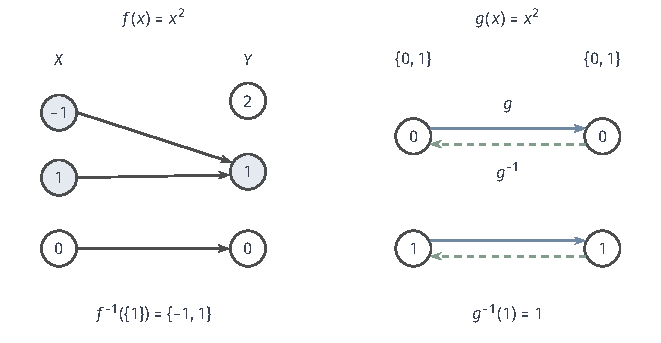
\includegraphics[width=112.0mm]{figures/01-mathematical-preliminaries-upper/01-mathematical-language-combinatorics-analysis-optimization/tikz/prelim-preimage-inverse/figure.pdf}
  \caption{原像与逆映射回答不同问题。左侧$f:\{-1,0,1\}\to\{0,1,2\}$按平方取值，
  标出的$1$有两个原输入，$2$没有原输入；原像$f^{-1}(\{1\})=\{-1,1\}$仍有定义。
  右侧将定义域与陪域都限制为$\{0,1\}$得到双射$g$，实线表示正向求值，虚线表示
  逆映射，因而$g^{-1}(1)=1$是一个元素。两侧均为精确的有限映射。}
  \label{fig:prelim-preimage-inverse}
\end{figure}

双射复合后的反求需要倒转次序。若$f:X\to Y$与$g:Y\to Z$都是双射，
先撤销$g$，再撤销$f$，有
\begin{equation}
 (g\circ f)^{-1}=f^{-1}\circ g^{-1}.
 \label{eq:prelim-inverse-composition}
\end{equation}
验证时分别代入$x\in X$与$z\in Z$：
\[
 \begin{aligned}
 f^{-1}(g^{-1}(g(f(x))))&=x,\\
 g(f(f^{-1}(g^{-1}(z))))&=z.
 \end{aligned}
\]
例如取双射$f:[0,\infty)\to[0,\infty)$、$f(x)=x^2$与$g:[0,\infty)\to[1,\infty)$、$g(u)=u+1$，
复合$g\circ f$先平方、再加$1$，把非负数$x$变成$z=x^2+1$。
反求时次序倒转：先减$1$、再开平方，得到$x=\sqrt{z-1}$，其定义域为$[1,\infty)$。

\subsection{函数族与参数化}
\label{sec:prelim-function-families}

\paragraph{函数族}
回到本章开头的预测问题。我们事先并不知道哪条规则最合适，通常先划定一批候选规则，再从中挑选。
这批候选规则本身是一个集合，它的元素是整个函数。
具有同一定义域和陪域的一组函数组成函数族（family of functions）。

例如，形如$f(x)=ax+b$的函数称为一元仿射函数（affine function），所有这样的函数组成
\[
 \mathcal F=\{f_{a,b}:\mathbb R\to\mathbb R:\ f_{a,b}(x)=ax+b,\ (a,b)\in\mathbb R^2\}.
\]
族中的每个元素是一整个函数。取$(a,b)=(2,1)$得到函数$f_{2,1}(x)=2x+1$；
再取输入$x=3$，才得到一个函数值$f_{2,1}(3)=7$。

\paragraph{函数参数化}
用参数为函数族中的函数编号，称为参数化（parameterization）。
一般写成$\theta\mapsto f_\theta$，其中$\theta$属于参数集合$\Theta$，
$f_\theta:X\to Y$是相应的函数。
映射$\theta\mapsto f_\theta$的输入是参数，输出是函数；函数$f_\theta$自身的输入仍是$x$。
在上例中，$\theta=(a,b)$指定一条直线，而$x$指定在直线上的哪个位置求值。
参数化把“在函数中挑选”改写为“在参数集合中挑选”；参数集合通常是$\mathbb R^2$这样熟悉的集合，
便于后续用数值方法比较和调整。

\paragraph{函数参数化的可识别性}
不同参数可能表示同一个函数，所以参数与函数未必一一对应。能否由函数反过来确定参数，取决于下面的条件。
\begin{definition}[函数参数化的可识别性]
\label{def:prelim-identifiable-parameterization}
给定参数集合$\Theta$与函数族$\{f_\theta:X\to Y:\theta\in\Theta\}$。
若$f_\theta=f_{\theta'}$蕴含$\theta=\theta'$，即$\theta\mapsto f_\theta$为单射，
则称这一函数参数化可识别（identifiable）；也就是说，完整函数唯一确定其参数。
否则称为不可识别。
\end{definition}
这里比较的是整个定义域上的函数，而非几个位置的函数值。
例如仿射函数族中$b=f_{a,b}(0)$、$a=f_{a,b}(1)-f_{a,b}(0)$，
所以完整函数唯一确定$(a,b)$，这一参数化可识别。若只观察$x=0$处的函数值，则只能确定$b$，
不能确定$a$。可见，有限个观测是否足以确定参数，与参数化是否可识别是两个不同的问题。

\Needspace{11\baselineskip}
\begin{example}[参数不同而函数相同]
\label{ex:prelim-nonidentifiable-parameterization}
考虑参数化函数
\[
  f_{a,b}:\mathbb{R}\to\mathbb{R},
  \qquad
  f_{a,b}(x)=abx,
  \qquad
  (a,b)\in\mathbb{R}^2.
\]
参数$(1,2)$与$(2,1)$不同，却对每个$x$给出相同的函数值。更一般地，只要$c\neq0$，
$(ca,b/c)$与$(a,b)$就表示同一个函数。从完整的输入输出关系可以确定乘积$ab$（例如取$x=1$，有$ab=f_{a,b}(1)$），
却不能分别确定$a$和$b$。这是参数化本身不可识别，而不是计算精度不足。
\end{example}


图~\ref{fig:vol1-add-parameter-function-value}把“由参数得到函数”和“由函数得到函数值”这两层操作分开：三组不同参数先汇入同一条完整规则，然后才在指定的$x$处求值。
\begin{figure}[!htb]
  \centering
  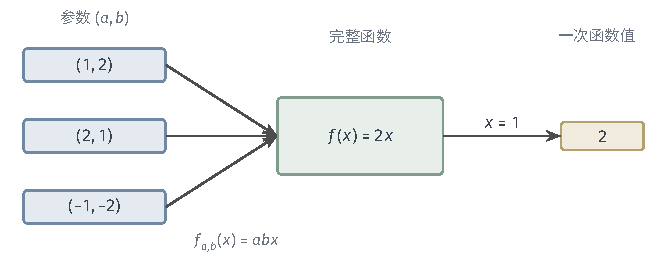
\includegraphics[width=112mm]{figures/01-mathematical-preliminaries-upper/00-shared/tikz/mathematical-language-combinatorics-analysis-optimization-comprehension-additions/parameter-function-value.pdf}
  \caption{参数化$f_{a,b}(x)=abx$中的三层对象。参数$(1,2),(2,1),(-1,-2)$的乘积均为$2$，所以它们表示同一个函数$f(x)=2x$；再指定$x=1$，才得到一次求值结果$2$。多组参数汇入同一完整函数，正是不可识别性。}
  \label{fig:vol1-add-parameter-function-value}
\end{figure}

不可识别的参数可以用前面的等价关系整理。规定$\theta\sim\theta'$当且仅当$f_\theta=f_{\theta'}$，
就得到参数集合上的等价关系：函数相等本身是反身、对称、传递的，三条性质直接继承。
每个等价类收集同一个函数的全部参数表示；在$f_{a,b}(x)=abx$中，$(a,b)$所在的等价类是满足$a'b'=ab$的全部参数$(a',b')$。

把每个等价类对应到它所表示的函数，就得到从商集$\Theta/{\sim}$到函数族$\{f_\theta:\theta\in\Theta\}$的双射。
参数化可识别，恰好意味着每个等价类只含一个参数。
换言之，函数族中的元素按函数区分，参数则可能为同一个函数保留多种表示。

\subsection{实值函数的界与极值}
\label{sec:prelim-optimal-values-errors}

从候选函数中挑选时，常把每个候选的优劣写成一个实数，例如预测误差，再寻找使它最小的候选。
这就要求讨论一个实值函数能取到多小的值、最小值是否真的取得。
函数值组成实数集合，而实数的通常大小$\leq$是全序。下面先把偏序集合中的界与确界用于实数，
说明保证确界存在的实数完备性，再把这些概念用于函数。

\paragraph{上界与下界}
设$A\subseteq\mathbb R$非空。若$a\leq M$对每个$a\in A$成立，
就称$M$为$A$的上界（upper bound）；若$m\leq a$对每个$a\in A$成立，
就称$m$为下界（lower bound）。这正是前面偏序集合中上界、下界的定义在$(\mathbb R,\leq)$中的情形。
存在上界称为上有界，存在下界称为下有界，两者都有称为有界。
例如$(0,1)$有上界$1,2$，也有下界$0,-1$。界不必是集合中的元素，也不唯一。

\paragraph{上确界与下确界}
上界中的最小者称为\term{上确界}（supremum），记作$\sup A$；
下界中的最大者称为\term{下确界}（infimum），记作$\inf A$。
例如$\sup(0,1)=1$、$\inf(0,1)=0$，两个确界都不属于$(0,1)$。

上确界$\beta$不仅要满足$a\leq\beta$对所有$a\in A$成立，
还要满足每个$\varepsilon>0$都存在$a\in A$使$a>\beta-\varepsilon$。
后一个条件说明，任何比$\beta$小的数都不是上界。
下确界$\alpha$类似地满足$\alpha\leq a$对所有$a\in A$成立，且每个$\varepsilon>0$都存在$a\in A$
使$a<\alpha+\varepsilon$。

上界有无限多个，其中是否真有最小的一个，并不能从定义直接看出。
本书把下面的性质作为实数的基本性质使用，称为实数的完备性（也称确界原理）：
非空上有界实数集合有实数上确界，非空下有界实数集合有实数下确界。
有理数没有这一性质：集合$\{q\in\mathbb Q:q^2<2\}$在有理数中有上界（例如$2$），
但它在实数中的上确界是$\sqrt2$，而$\sqrt2$不是有理数。于是每个有理上界都严格大于$\sqrt2$，
在它与$\sqrt2$之间总还有更小的有理上界，所以在有理数中找不到最小的上界。
实数补上了这样的“空隙”，后面关于极限存在的结论都要用到这一点。

\paragraph{函数的有界性}
对非空定义域$X$上的实值函数$f:X\to\mathbb R$，讨论其有界性就是讨论值域$f(X)$的有界性。
例如$f(x)=x$在$(0,1)$上有界，在$\mathbb R$上则既无上界也无下界。
值域的确界简记为
\[
 \inf_{x\in X}f(x)=\inf f(X),\qquad
 \sup_{x\in X}f(x)=\sup f(X).
\]
若$f(X)$无下界，约定其下确界为$-\infty$；若无上界，约定其上确界为$+\infty$。
这两个符号表示没有有限的界，不是实值函数实际取到的数。

\paragraph{最小值与最小点}
若存在$x^\star\in X$使
\[
 \forall x\in X,\qquad f(x^\star)\leq f(x),
\]
则称$x^\star$为\term{全局最小点}（global minimizer），$f(x^\star)$为最小值。
符号$\forall$读作“对所有”，这里要求与定义域内的每个函数值比较。
最小值记作$\min_{x\in X}f(x)$；全部最小点组成的集合记作
\[
 \argmin_{x\in X}f(x)
 =\{x\in X:\ f(x)\leq f(z)\text{ 对所有 }z\in X\}.
\]
$\min$给出一个数，$\argmin$给出输入的集合；若不存在最小点，后一个集合为空。

最小值存在时必等于下确界：$f(x^\star)$不超过每个函数值，所以是值域的一个下界；
任何下界$m$都满足$m\leq f(x^\star)$，因为$f(x^\star)$本身就是一个函数值。
所以$f(x^\star)$是最大的下界。反过来，下确界存在却未必被取得。
例如$f(x)=x$在$(0,1)$上的下确界为$0$，但没有最小点，
因为任意允许的$x$都有更小的允许输入$x/2$。

\paragraph{最大值与最大点}
若存在$x^\star\in X$使$f(x^\star)\geq f(x)$对所有$x\in X$成立，
则称$x^\star$为全局最大点，$f(x^\star)$为最大值。
最大值记作$\max_{x\in X}f(x)$，全部最大点组成
\[
 \argmax_{x\in X}f(x)
 =\{x\in X:\ f(x)\geq f(z)\text{ 对所有 }z\in X\}.
\]
与最小值的论证对称，最大值存在时等于上确界。函数$f(x)=x$在$(0,1)$上没有最大值；
将定义域换为$[0,1]$后，最大值为$1$、最大点为$1$，最小值为$0$、最小点为$0$。

\begin{example}[同一个最优值可以对应多个输入]
\label{ex:prelim-optimal-value-versus-points}
令$X=[-2,2]$，$f(x)=(x^2-1)^2$。平方非负，且$x=\pm1$都使它为零，所以
\[
  \min_{x\in X}f(x)=\inf_{x\in X}f(x)=0,\qquad
  \argmin_{x\in X}f(x)=\{-1,1\}.
\]
又因为$0\leq x^2\leq4$，有$|x^2-1|\leq3$，于是$f(x)\leq9$，等号恰在$x=\pm2$
处成立。因此最大值为$9$，最大点集合为$\{-2,2\}$。最小值是一个数，不会因为有两个
最小点就变成两个最小值；最优点是否唯一是另一个问题。
\end{example}

图~\ref{fig:prelim-minimum-infimum}固定表达式$f(x)=x$，比较它在$(0,1)$与$[0,1]$上定义的两个函数。
两侧的函数值都以$0$为下确界；右侧把$x=0$纳入定义域后，这个下确界才由某个输入取得。
区别的关键在于边界点是否属于定义域，而不在于两条曲线是否趋向同一个高度。

\begin{figure}[htbp]
  \centering
  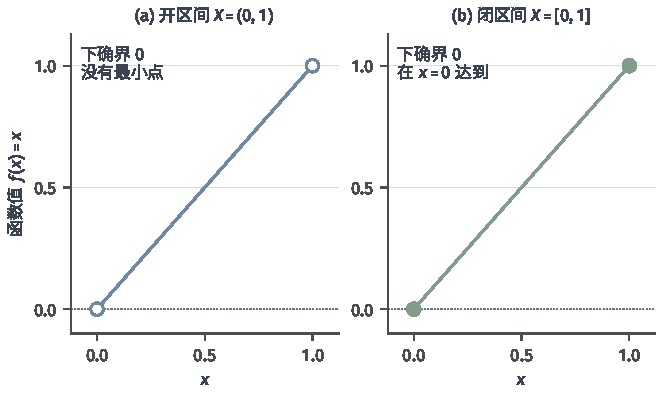
\includegraphics[width=112.0mm]{figures/01-mathematical-preliminaries-upper/01-mathematical-language-combinatorics-analysis-optimization/matplotlib/prelim-minimum-infimum/figure.pdf}
  \caption{同一求值表达式$f(x)=x$在两个定义域上的边界对照。左图定义域为$(0,1)$，空心端点不属于图像，函数值可任意接近$0$，却不能取到；右图定义域为$[0,1]$，实心端点$(0,0)$达到下确界。两图的下确界相同，最小点是否存在取决于可行端点是否保留。图为解析教学示例。}
  \label{fig:prelim-minimum-infimum}
\end{figure}
\FloatBarrier

\section{本章小结}
\label{sec:prelim-sets-functions-summary}

回到开头的四个问题：允许的输入和输出由集合规定，输入到输出的对应由函数描述，
候选规则由函数族与参数化编号、由界与最值比较，多次观测的数值则由索引族编号、由有限和与有限积汇总。

集合的运算满足交换、结合、分配与De Morgan律，两个集合相等可以拆成双向包含来证明。
二元关系把满足条件的有序对收集为笛卡尔积的子集；
关系的自反、对称与传递闭包分别补入对应性质所必需的有序对。
等价关系恰好对应集合的划分，偏序关系允许部分对象互不可比；最小元与极小元、界与集合内的最值需要分别判断。
索引族保留各项的编号与重复出现，集合族的并与交把两个集合的运算推广到任意多个。
有限和、有限积和递推描述这些项怎样汇总或生成，数学归纳法确认由递推得到的通项对每一步都成立，
有限几何和与裂项求和则是后文估计无限求和的起点。

函数是每个输入恰有一个输出的关系：像与原像分别沿输出和输入方向收集对象，原像保持并、交与补，
逆映射则要求函数为双射，也就是可以双向撤销；复合满足结合律，但一般不能交换次序。
函数族以整个函数为元素，参数化为这些函数编号，不同编号可以对应同一个函数。
比较候选函数时，确界原理保证非空定义域上有界函数的值域有上、下确界，但最值是否取得还要另外判断。

这些对象与记号是后续讨论的共同起点：第~\ref{chap:combinatorics}章研究集合的有限计数与基数比较，
第~\ref{chap:function-limits}章研究极限；第~\ref{chap:linear-operations}章起的线性空间部分把有限组数值排成向量与矩阵，
并在其上建立线性运算；随后第~\ref{chap:univariate-differentiation}章、第~\ref{chap:univariate-integration}章和第~\ref{chap:multivariate-calculus}章分别研究一元函数的微分、一元函数的积分与多元微积分。
